% Created by tikzDevice version 0.12.6 on 2026-08-08 13:32:28
% !TEX encoding = UTF-8 Unicode
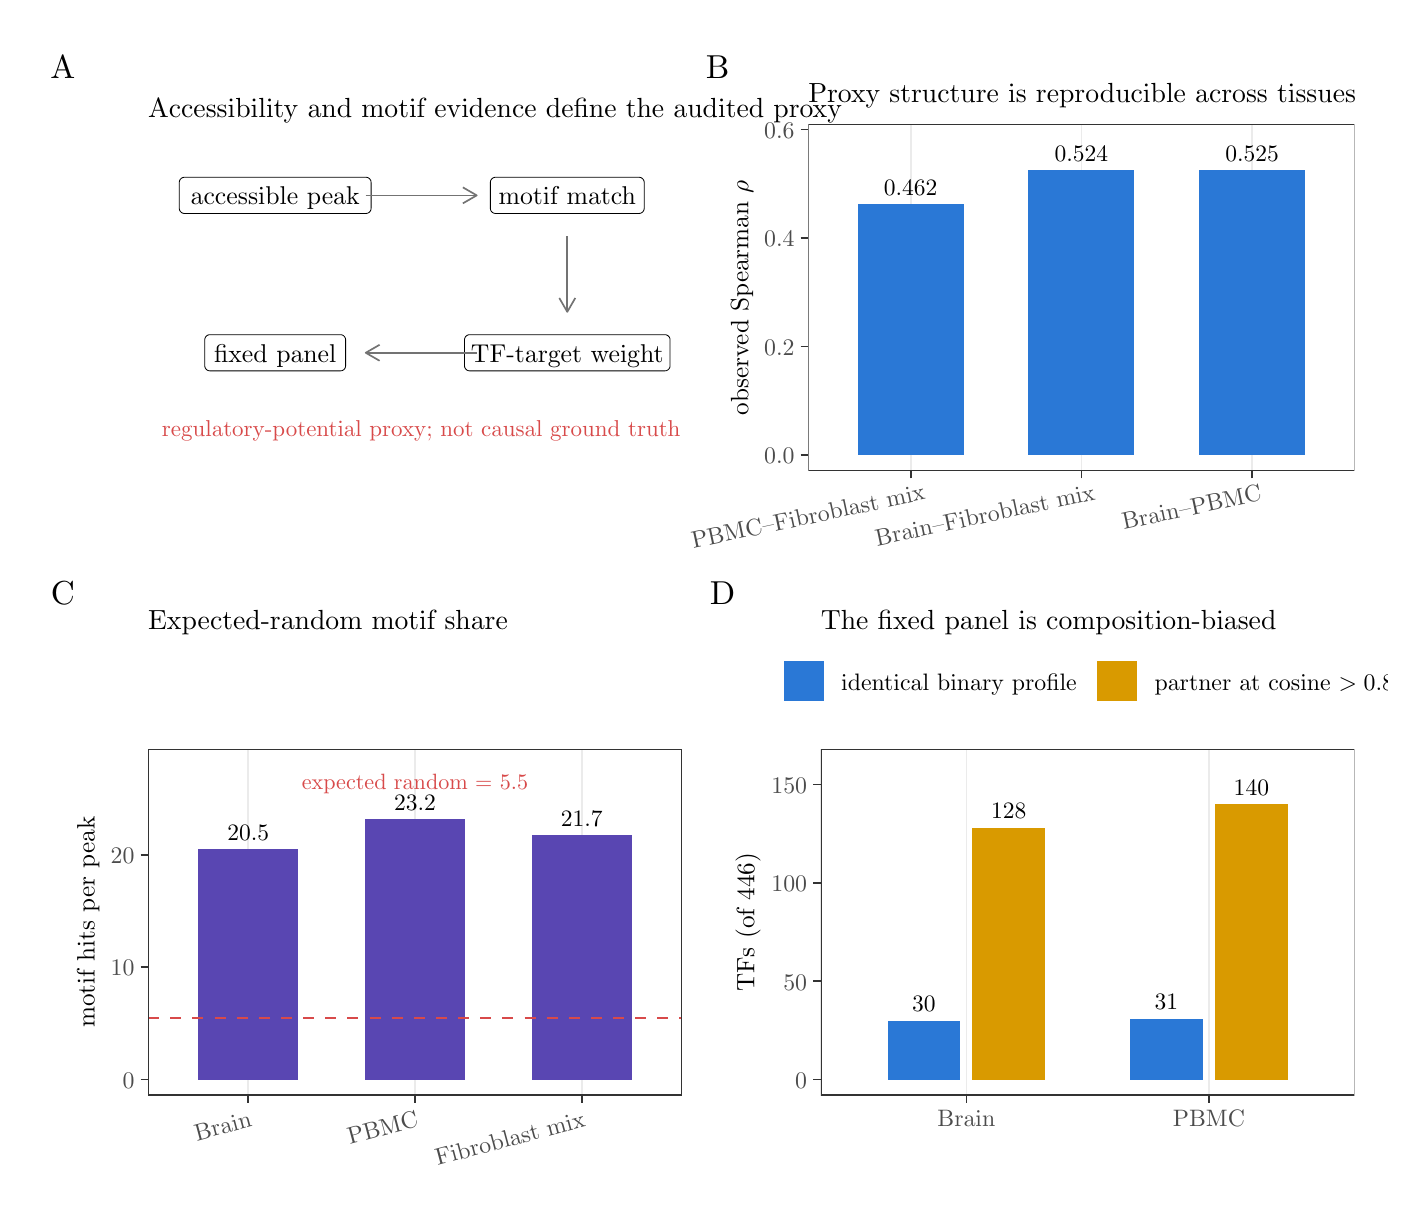
\begin{tikzpicture}[x=1pt,y=1pt]
\definecolor{fillColor}{RGB}{255,255,255}
\path[use as bounding box,fill=fillColor,fill opacity=0.00] (0,0) rectangle (491.44,419.17);
\begin{scope}
\path[clip] (  0.00,  0.00) rectangle (491.44,419.17);
\definecolor{drawColor}{RGB}{255,255,255}
\definecolor{fillColor}{RGB}{255,255,255}

\path[draw=drawColor,line width= 0.6pt,line join=round,line cap=round,fill=fillColor] ( -0.00,  0.00) rectangle (491.44,419.17);
\end{scope}
\begin{scope}
\path[clip] (  4.00,224.91) rectangle (240.90,415.17);

\path[] (  4.00,224.91) rectangle (240.90,415.17);
\end{scope}
\begin{scope}
\path[clip] (240.90,224.91) rectangle (485.44,415.17);
\definecolor{drawColor}{RGB}{255,255,255}
\definecolor{fillColor}{RGB}{255,255,255}

\path[draw=drawColor,line width= 0.6pt,line join=round,line cap=round,fill=fillColor] (240.90,224.91) rectangle (485.44,415.17);
\end{scope}
\begin{scope}
\path[clip] (  0.00,  0.00) rectangle (491.44,419.17);
\definecolor{drawColor}{RGB}{0,0,0}
\definecolor{fillColor}{RGB}{255,255,255}

\path[draw=drawColor,line width= 0.3pt,line join=round,line cap=round,fill=fillColor] ( 56.64,352.04) --
	(122.24,352.04) --
	(122.17,352.04) --
	(122.47,352.05) --
	(122.76,352.11) --
	(123.04,352.22) --
	(123.29,352.37) --
	(123.52,352.55) --
	(123.72,352.78) --
	(123.88,353.03) --
	(124.00,353.30) --
	(124.07,353.59) --
	(124.09,353.89) --
	(124.09,353.89) --
	(124.09,363.25) --
	(124.09,363.25) --
	(124.07,363.55) --
	(124.00,363.84) --
	(123.88,364.11) --
	(123.72,364.36) --
	(123.52,364.58) --
	(123.29,364.77) --
	(123.04,364.92) --
	(122.76,365.03) --
	(122.47,365.09) --
	(122.24,365.10) --
	( 56.64,365.10) --
	( 56.86,365.09) --
	( 56.56,365.10) --
	( 56.27,365.06) --
	( 55.98,364.98) --
	( 55.71,364.85) --
	( 55.47,364.68) --
	( 55.25,364.48) --
	( 55.07,364.24) --
	( 54.94,363.98) --
	( 54.84,363.69) --
	( 54.79,363.40) --
	( 54.79,363.25) --
	( 54.79,353.89) --
	( 54.79,354.04) --
	( 54.79,353.74) --
	( 54.84,353.45) --
	( 54.94,353.16) --
	( 55.07,352.90) --
	( 55.25,352.66) --
	( 55.47,352.46) --
	( 55.71,352.29) --
	( 55.98,352.16) --
	( 56.27,352.08) --
	( 56.56,352.04) --
	cycle;
\end{scope}
\begin{scope}
\path[clip] (  0.00,  0.00) rectangle (491.44,419.17);
\definecolor{drawColor}{RGB}{0,0,0}

\node[text=drawColor,anchor=base,inner sep=0pt, outer sep=0pt, scale=  0.93] at ( 89.44,355.12) {accessible peak};
\end{scope}
\begin{scope}
\path[clip] (  0.00,  0.00) rectangle (491.44,419.17);
\definecolor{drawColor}{RGB}{0,0,0}
\definecolor{fillColor}{RGB}{255,255,255}

\path[draw=drawColor,line width= 0.3pt,line join=round,line cap=round,fill=fillColor] (169.05,352.04) --
	(220.93,352.04) --
	(220.85,352.04) --
	(221.15,352.05) --
	(221.44,352.11) --
	(221.72,352.22) --
	(221.98,352.37) --
	(222.21,352.55) --
	(222.40,352.78) --
	(222.56,353.03) --
	(222.68,353.30) --
	(222.75,353.59) --
	(222.78,353.89) --
	(222.78,353.89) --
	(222.78,363.25) --
	(222.78,363.25) --
	(222.75,363.55) --
	(222.68,363.84) --
	(222.56,364.11) --
	(222.40,364.36) --
	(222.21,364.58) --
	(221.98,364.77) --
	(221.72,364.92) --
	(221.44,365.03) --
	(221.15,365.09) --
	(220.93,365.10) --
	(169.05,365.10) --
	(169.27,365.09) --
	(168.97,365.10) --
	(168.67,365.06) --
	(168.39,364.98) --
	(168.12,364.85) --
	(167.87,364.68) --
	(167.66,364.48) --
	(167.48,364.24) --
	(167.34,363.98) --
	(167.25,363.69) --
	(167.20,363.40) --
	(167.19,363.25) --
	(167.19,353.89) --
	(167.20,354.04) --
	(167.20,353.74) --
	(167.25,353.45) --
	(167.34,353.16) --
	(167.48,352.90) --
	(167.66,352.66) --
	(167.87,352.46) --
	(168.12,352.29) --
	(168.39,352.16) --
	(168.67,352.08) --
	(168.97,352.04) --
	cycle;
\end{scope}
\begin{scope}
\path[clip] (  0.00,  0.00) rectangle (491.44,419.17);
\definecolor{drawColor}{RGB}{0,0,0}

\node[text=drawColor,anchor=base,inner sep=0pt, outer sep=0pt, scale=  0.93] at (194.99,355.12) {motif match};
\end{scope}
\begin{scope}
\path[clip] (  0.00,  0.00) rectangle (491.44,419.17);
\definecolor{drawColor}{RGB}{0,0,0}
\definecolor{fillColor}{RGB}{255,255,255}

\path[draw=drawColor,line width= 0.3pt,line join=round,line cap=round,fill=fillColor] (159.70,295.16) --
	(230.27,295.16) --
	(230.20,295.16) --
	(230.49,295.17) --
	(230.79,295.23) --
	(231.06,295.34) --
	(231.32,295.49) --
	(231.55,295.67) --
	(231.75,295.90) --
	(231.91,296.15) --
	(232.03,296.42) --
	(232.10,296.71) --
	(232.12,297.01) --
	(232.12,297.01) --
	(232.12,306.37) --
	(232.12,306.37) --
	(232.10,306.67) --
	(232.03,306.96) --
	(231.91,307.23) --
	(231.75,307.48) --
	(231.55,307.70) --
	(231.32,307.89) --
	(231.06,308.04) --
	(230.79,308.15) --
	(230.49,308.21) --
	(230.27,308.22) --
	(159.70,308.22) --
	(159.92,308.21) --
	(159.63,308.22) --
	(159.33,308.18) --
	(159.04,308.10) --
	(158.77,307.97) --
	(158.53,307.80) --
	(158.31,307.60) --
	(158.14,307.36) --
	(158.00,307.10) --
	(157.90,306.81) --
	(157.86,306.52) --
	(157.85,306.37) --
	(157.85,297.01) --
	(157.86,297.16) --
	(157.86,296.86) --
	(157.90,296.57) --
	(158.00,296.28) --
	(158.14,296.02) --
	(158.31,295.78) --
	(158.53,295.58) --
	(158.77,295.41) --
	(159.04,295.28) --
	(159.33,295.20) --
	(159.63,295.16) --
	cycle;
\end{scope}
\begin{scope}
\path[clip] (  0.00,  0.00) rectangle (491.44,419.17);
\definecolor{drawColor}{RGB}{0,0,0}

\node[text=drawColor,anchor=base,inner sep=0pt, outer sep=0pt, scale=  0.93] at (194.99,298.24) {TF-target weight};
\end{scope}
\begin{scope}
\path[clip] (  0.00,  0.00) rectangle (491.44,419.17);
\definecolor{drawColor}{RGB}{0,0,0}
\definecolor{fillColor}{RGB}{255,255,255}

\path[draw=drawColor,line width= 0.3pt,line join=round,line cap=round,fill=fillColor] ( 65.85,295.16) --
	(113.04,295.16) --
	(112.96,295.16) --
	(113.26,295.17) --
	(113.55,295.23) --
	(113.83,295.34) --
	(114.09,295.49) --
	(114.32,295.67) --
	(114.51,295.90) --
	(114.67,296.15) --
	(114.79,296.42) --
	(114.86,296.71) --
	(114.89,297.01) --
	(114.89,297.01) --
	(114.89,306.37) --
	(114.89,306.37) --
	(114.86,306.67) --
	(114.79,306.96) --
	(114.67,307.23) --
	(114.51,307.48) --
	(114.32,307.70) --
	(114.09,307.89) --
	(113.83,308.04) --
	(113.55,308.15) --
	(113.26,308.21) --
	(113.04,308.22) --
	( 65.85,308.22) --
	( 66.07,308.21) --
	( 65.77,308.22) --
	( 65.47,308.18) --
	( 65.19,308.10) --
	( 64.92,307.97) --
	( 64.67,307.80) --
	( 64.46,307.60) --
	( 64.28,307.36) --
	( 64.14,307.10) --
	( 64.05,306.81) --
	( 64.00,306.52) --
	( 63.99,306.37) --
	( 63.99,297.01) --
	( 64.00,297.16) --
	( 64.00,296.86) --
	( 64.05,296.57) --
	( 64.14,296.28) --
	( 64.28,296.02) --
	( 64.46,295.78) --
	( 64.67,295.58) --
	( 64.92,295.41) --
	( 65.19,295.28) --
	( 65.47,295.20) --
	( 65.77,295.16) --
	cycle;
\end{scope}
\begin{scope}
\path[clip] (  0.00,  0.00) rectangle (491.44,419.17);
\definecolor{drawColor}{RGB}{0,0,0}

\node[text=drawColor,anchor=base,inner sep=0pt, outer sep=0pt, scale=  0.93] at ( 89.44,298.24) {fixed panel};
\end{scope}
\begin{scope}
\path[clip] (  0.00,  0.00) rectangle (491.44,419.17);
\definecolor{drawColor}{gray}{0.45}

\path[draw=drawColor,line width= 0.6pt,line join=round] (122.16,358.57) -- (162.27,358.57);

\path[draw=drawColor,line width= 0.6pt,line join=round] (157.26,355.68) --
	(162.27,358.57) --
	(157.26,361.46);

\path[draw=drawColor,line width= 0.6pt,line join=round] (194.99,343.78) -- (194.99,316.48);

\path[draw=drawColor,line width= 0.6pt,line join=round] (192.09,321.49) --
	(194.99,316.48) --
	(197.88,321.49);

\path[draw=drawColor,line width= 0.6pt,line join=round] (162.27,301.69) -- (122.16,301.69);

\path[draw=drawColor,line width= 0.6pt,line join=round] (127.17,304.58) --
	(122.16,301.69) --
	(127.17,298.80);
\definecolor{drawColor}{RGB}{216,74,74}

\node[text=drawColor,anchor=base,inner sep=0pt, outer sep=0pt, scale=  0.83] at (142.21,271.32) {regulatory-potential proxy; not causal ground truth};
\end{scope}
\begin{scope}
\path[clip] (  0.00,  0.00) rectangle (491.44,419.17);
\definecolor{drawColor}{RGB}{0,0,0}

\node[text=drawColor,anchor=base west,inner sep=0pt, outer sep=0pt, scale=  1.00] at ( 43.53,386.54) {Accessibility and motif evidence define the audited proxy};
\end{scope}
\begin{scope}
\path[clip] (  0.00,  0.00) rectangle (491.44,419.17);
\definecolor{drawColor}{RGB}{0,0,0}

\node[text=drawColor,anchor=base,inner sep=0pt, outer sep=0pt, scale=  1.20] at ( 12.74,400.86) {A};
\end{scope}
\begin{scope}
\path[clip] (282.07,259.03) rectangle (479.44,384.17);
\definecolor{fillColor}{RGB}{255,255,255}

\path[fill=fillColor] (282.07,259.03) rectangle (479.44,384.17);
\definecolor{drawColor}{gray}{0.92}

\path[draw=drawColor,line width= 0.6pt,line join=round] (319.07,259.03) --
	(319.07,384.17);

\path[draw=drawColor,line width= 0.6pt,line join=round] (380.75,259.03) --
	(380.75,384.17);

\path[draw=drawColor,line width= 0.6pt,line join=round] (442.43,259.03) --
	(442.43,384.17);
\definecolor{fillColor}{RGB}{42,120,214}

\path[fill=fillColor] (423.31,264.72) rectangle (461.55,367.66);

\path[fill=fillColor] (361.63,264.72) rectangle (399.87,367.59);

\path[fill=fillColor] (299.95,264.72) rectangle (338.19,355.40);
\definecolor{drawColor}{RGB}{0,0,0}

\node[text=drawColor,anchor=base,inner sep=0pt, outer sep=0pt, scale=  0.85] at (442.43,370.82) {0.525};

\node[text=drawColor,anchor=base,inner sep=0pt, outer sep=0pt, scale=  0.85] at (380.75,370.75) {0.524};

\node[text=drawColor,anchor=base,inner sep=0pt, outer sep=0pt, scale=  0.85] at (319.07,358.56) {0.462};
\definecolor{drawColor}{gray}{0.20}

\path[draw=drawColor,line width= 0.6pt,line join=round,line cap=round] (282.07,259.03) rectangle (479.44,384.17);
\end{scope}
\begin{scope}
\path[clip] (  0.00,  0.00) rectangle (491.44,419.17);
\definecolor{drawColor}{gray}{0.30}

\node[text=drawColor,anchor=base east,inner sep=0pt, outer sep=0pt, scale=  0.86] at (277.12,261.52) {0.0};

\node[text=drawColor,anchor=base east,inner sep=0pt, outer sep=0pt, scale=  0.86] at (277.12,300.75) {0.2};

\node[text=drawColor,anchor=base east,inner sep=0pt, outer sep=0pt, scale=  0.86] at (277.12,339.98) {0.4};

\node[text=drawColor,anchor=base east,inner sep=0pt, outer sep=0pt, scale=  0.86] at (277.12,379.20) {0.6};
\end{scope}
\begin{scope}
\path[clip] (  0.00,  0.00) rectangle (491.44,419.17);
\definecolor{drawColor}{gray}{0.20}

\path[draw=drawColor,line width= 0.6pt,line join=round] (279.32,264.72) --
	(282.07,264.72);

\path[draw=drawColor,line width= 0.6pt,line join=round] (279.32,303.95) --
	(282.07,303.95);

\path[draw=drawColor,line width= 0.6pt,line join=round] (279.32,343.17) --
	(282.07,343.17);

\path[draw=drawColor,line width= 0.6pt,line join=round] (279.32,382.40) --
	(282.07,382.40);
\end{scope}
\begin{scope}
\path[clip] (  0.00,  0.00) rectangle (491.44,419.17);
\definecolor{drawColor}{gray}{0.20}

\path[draw=drawColor,line width= 0.6pt,line join=round] (319.07,256.28) --
	(319.07,259.03);

\path[draw=drawColor,line width= 0.6pt,line join=round] (380.75,256.28) --
	(380.75,259.03);

\path[draw=drawColor,line width= 0.6pt,line join=round] (442.43,256.28) --
	(442.43,259.03);
\end{scope}
\begin{scope}
\path[clip] (  0.00,  0.00) rectangle (491.44,419.17);
\definecolor{drawColor}{gray}{0.30}

\node[text=drawColor,rotate= 12.00,anchor=base east,inner sep=0pt, outer sep=0pt, scale=  0.86] at (324.62,248.72) {PBMC--Fibroblast mix};

\node[text=drawColor,rotate= 12.00,anchor=base east,inner sep=0pt, outer sep=0pt, scale=  0.86] at (386.04,248.67) {Brain--Fibroblast mix};

\node[text=drawColor,rotate= 12.00,anchor=base east,inner sep=0pt, outer sep=0pt, scale=  0.86] at (446.30,248.37) {Brain--PBMC};
\end{scope}
\begin{scope}
\path[clip] (  0.00,  0.00) rectangle (491.44,419.17);
\definecolor{drawColor}{RGB}{0,0,0}

\node[text=drawColor,rotate= 90.00,anchor=base,inner sep=0pt, outer sep=0pt, scale=  0.91] at (260.39,321.60) {observed Spearman $\rho$};
\end{scope}
\begin{scope}
\path[clip] (  0.00,  0.00) rectangle (491.44,419.17);
\definecolor{drawColor}{RGB}{0,0,0}

\node[text=drawColor,anchor=base west,inner sep=0pt, outer sep=0pt, scale=  1.00] at (282.07,392.04) {Proxy structure is reproducible across tissues};
\end{scope}
\begin{scope}
\path[clip] (  0.00,  0.00) rectangle (491.44,419.17);
\definecolor{drawColor}{RGB}{0,0,0}

\node[text=drawColor,anchor=base,inner sep=0pt, outer sep=0pt, scale=  1.20] at (249.28,400.86) {B};
\end{scope}
\begin{scope}
\path[clip] (  4.00,  3.00) rectangle (242.35,224.91);
\definecolor{drawColor}{RGB}{255,255,255}
\definecolor{fillColor}{RGB}{255,255,255}

\path[draw=drawColor,line width= 0.6pt,line join=round,line cap=round,fill=fillColor] (  4.00,  3.00) rectangle (242.35,224.91);
\end{scope}
\begin{scope}
\path[clip] (242.35,  3.00) rectangle (485.44,224.91);
\definecolor{drawColor}{RGB}{255,255,255}
\definecolor{fillColor}{RGB}{255,255,255}

\path[draw=drawColor,line width= 0.6pt,line join=round,line cap=round,fill=fillColor] (242.35,  3.00) rectangle (485.44,224.91);
\end{scope}
\begin{scope}
\path[clip] ( 43.53, 33.38) rectangle (236.35,158.51);
\definecolor{fillColor}{RGB}{255,255,255}

\path[fill=fillColor] ( 43.53, 33.38) rectangle (236.35,158.51);
\definecolor{drawColor}{gray}{0.92}

\path[draw=drawColor,line width= 0.6pt,line join=round] ( 79.68, 33.38) --
	( 79.68,158.51);

\path[draw=drawColor,line width= 0.6pt,line join=round] (139.94, 33.38) --
	(139.94,158.51);

\path[draw=drawColor,line width= 0.6pt,line join=round] (200.20, 33.38) --
	(200.20,158.51);
\definecolor{fillColor}{RGB}{89,70,178}

\path[fill=fillColor] ( 61.61, 39.06) rectangle ( 97.76,122.22);

\path[fill=fillColor] (121.86, 39.06) rectangle (158.02,133.25);

\path[fill=fillColor] (182.12, 39.06) rectangle (218.28,127.26);
\definecolor{drawColor}{RGB}{216,74,74}

\path[draw=drawColor,line width= 0.6pt,dash pattern=on 4pt off 4pt ,line join=round] ( 43.53, 61.41) -- (236.35, 61.41);
\definecolor{drawColor}{RGB}{0,0,0}

\node[text=drawColor,anchor=base,inner sep=0pt, outer sep=0pt, scale=  0.85] at ( 79.68,125.38) {20.5};

\node[text=drawColor,anchor=base,inner sep=0pt, outer sep=0pt, scale=  0.85] at (139.94,136.41) {23.2};

\node[text=drawColor,anchor=base,inner sep=0pt, outer sep=0pt, scale=  0.85] at (200.20,130.42) {21.7};
\definecolor{drawColor}{RGB}{216,74,74}

\node[text=drawColor,anchor=base,inner sep=0pt, outer sep=0pt, scale=  0.80] at (139.94,143.76) {expected random = 5.5};
\definecolor{drawColor}{gray}{0.20}

\path[draw=drawColor,line width= 0.6pt,line join=round,line cap=round] ( 43.53, 33.38) rectangle (236.35,158.51);
\end{scope}
\begin{scope}
\path[clip] (  0.00,  0.00) rectangle (491.44,419.17);
\definecolor{drawColor}{gray}{0.30}

\node[text=drawColor,anchor=base east,inner sep=0pt, outer sep=0pt, scale=  0.86] at ( 38.58, 35.87) {0};

\node[text=drawColor,anchor=base east,inner sep=0pt, outer sep=0pt, scale=  0.86] at ( 38.58, 76.50) {10};

\node[text=drawColor,anchor=base east,inner sep=0pt, outer sep=0pt, scale=  0.86] at ( 38.58,117.12) {20};
\end{scope}
\begin{scope}
\path[clip] (  0.00,  0.00) rectangle (491.44,419.17);
\definecolor{drawColor}{gray}{0.20}

\path[draw=drawColor,line width= 0.6pt,line join=round] ( 40.78, 39.06) --
	( 43.53, 39.06);

\path[draw=drawColor,line width= 0.6pt,line join=round] ( 40.78, 79.69) --
	( 43.53, 79.69);

\path[draw=drawColor,line width= 0.6pt,line join=round] ( 40.78,120.32) --
	( 43.53,120.32);
\end{scope}
\begin{scope}
\path[clip] (  0.00,  0.00) rectangle (491.44,419.17);
\definecolor{drawColor}{gray}{0.20}

\path[draw=drawColor,line width= 0.6pt,line join=round] ( 79.68, 30.63) --
	( 79.68, 33.38);

\path[draw=drawColor,line width= 0.6pt,line join=round] (139.94, 30.63) --
	(139.94, 33.38);

\path[draw=drawColor,line width= 0.6pt,line join=round] (200.20, 30.63) --
	(200.20, 33.38);
\end{scope}
\begin{scope}
\path[clip] (  0.00,  0.00) rectangle (491.44,419.17);
\definecolor{drawColor}{gray}{0.30}

\node[text=drawColor,rotate= 15.00,anchor=base east,inner sep=0pt, outer sep=0pt, scale=  0.86] at ( 81.34, 22.25) {Brain};

\node[text=drawColor,rotate= 15.00,anchor=base east,inner sep=0pt, outer sep=0pt, scale=  0.86] at (141.60, 22.25) {PBMC};

\node[text=drawColor,rotate= 15.00,anchor=base east,inner sep=0pt, outer sep=0pt, scale=  0.86] at (201.85, 22.25) {Fibroblast mix};
\end{scope}
\begin{scope}
\path[clip] (  0.00,  0.00) rectangle (491.44,419.17);
\definecolor{drawColor}{RGB}{0,0,0}

\node[text=drawColor,rotate= 90.00,anchor=base,inner sep=0pt, outer sep=0pt, scale=  0.91] at ( 24.22, 95.94) {motif hits per peak};
\end{scope}
\begin{scope}
\path[clip] (  0.00,  0.00) rectangle (491.44,419.17);
\definecolor{drawColor}{RGB}{0,0,0}

\node[text=drawColor,anchor=base west,inner sep=0pt, outer sep=0pt, scale=  1.00] at ( 43.53,201.78) {Expected-random motif share};
\end{scope}
\begin{scope}
\path[clip] (  0.00,  0.00) rectangle (491.44,419.17);
\definecolor{drawColor}{RGB}{0,0,0}

\node[text=drawColor,anchor=base,inner sep=0pt, outer sep=0pt, scale=  1.20] at ( 12.74,210.61) {C};
\end{scope}
\begin{scope}
\path[clip] (286.61, 33.38) rectangle (479.44,158.51);
\definecolor{fillColor}{RGB}{255,255,255}

\path[fill=fillColor] (286.61, 33.38) rectangle (479.44,158.51);
\definecolor{drawColor}{gray}{0.92}

\path[draw=drawColor,line width= 0.6pt,line join=round] (339.20, 33.38) --
	(339.20,158.51);

\path[draw=drawColor,line width= 0.6pt,line join=round] (426.85, 33.38) --
	(426.85,158.51);
\definecolor{fillColor}{RGB}{42,120,214}

\path[fill=fillColor] (310.71, 39.06) rectangle (337.01, 60.39);
\definecolor{fillColor}{RGB}{217,154,0}

\path[fill=fillColor] (341.39, 39.06) rectangle (367.68,130.07);
\definecolor{fillColor}{RGB}{42,120,214}

\path[fill=fillColor] (398.36, 39.06) rectangle (424.66, 61.11);
\definecolor{fillColor}{RGB}{217,154,0}

\path[fill=fillColor] (429.04, 39.06) rectangle (455.33,138.60);
\definecolor{drawColor}{RGB}{0,0,0}

\node[text=drawColor,anchor=base,inner sep=0pt, outer sep=0pt, scale=  0.85] at (323.86, 63.55) {30};

\node[text=drawColor,anchor=base,inner sep=0pt, outer sep=0pt, scale=  0.85] at (354.54,133.23) {128};

\node[text=drawColor,anchor=base,inner sep=0pt, outer sep=0pt, scale=  0.85] at (411.51, 64.26) {31};

\node[text=drawColor,anchor=base,inner sep=0pt, outer sep=0pt, scale=  0.85] at (442.19,141.76) {140};
\definecolor{drawColor}{gray}{0.20}

\path[draw=drawColor,line width= 0.6pt,line join=round,line cap=round] (286.61, 33.38) rectangle (479.44,158.51);
\end{scope}
\begin{scope}
\path[clip] (  0.00,  0.00) rectangle (491.44,419.17);
\definecolor{drawColor}{gray}{0.30}

\node[text=drawColor,anchor=base east,inner sep=0pt, outer sep=0pt, scale=  0.86] at (281.66, 35.87) {0};

\node[text=drawColor,anchor=base east,inner sep=0pt, outer sep=0pt, scale=  0.86] at (281.66, 71.42) {50};

\node[text=drawColor,anchor=base east,inner sep=0pt, outer sep=0pt, scale=  0.86] at (281.66,106.97) {100};

\node[text=drawColor,anchor=base east,inner sep=0pt, outer sep=0pt, scale=  0.86] at (281.66,142.52) {150};
\end{scope}
\begin{scope}
\path[clip] (  0.00,  0.00) rectangle (491.44,419.17);
\definecolor{drawColor}{gray}{0.20}

\path[draw=drawColor,line width= 0.6pt,line join=round] (283.86, 39.06) --
	(286.61, 39.06);

\path[draw=drawColor,line width= 0.6pt,line join=round] (283.86, 74.61) --
	(286.61, 74.61);

\path[draw=drawColor,line width= 0.6pt,line join=round] (283.86,110.16) --
	(286.61,110.16);

\path[draw=drawColor,line width= 0.6pt,line join=round] (283.86,145.71) --
	(286.61,145.71);
\end{scope}
\begin{scope}
\path[clip] (  0.00,  0.00) rectangle (491.44,419.17);
\definecolor{drawColor}{gray}{0.20}

\path[draw=drawColor,line width= 0.6pt,line join=round] (339.20, 30.63) --
	(339.20, 33.38);

\path[draw=drawColor,line width= 0.6pt,line join=round] (426.85, 30.63) --
	(426.85, 33.38);
\end{scope}
\begin{scope}
\path[clip] (  0.00,  0.00) rectangle (491.44,419.17);
\definecolor{drawColor}{gray}{0.30}

\node[text=drawColor,anchor=base,inner sep=0pt, outer sep=0pt, scale=  0.86] at (339.20, 22.03) {Brain};

\node[text=drawColor,anchor=base,inner sep=0pt, outer sep=0pt, scale=  0.86] at (426.85, 22.03) {PBMC};
\end{scope}
\begin{scope}
\path[clip] (  0.00,  0.00) rectangle (491.44,419.17);
\definecolor{drawColor}{RGB}{0,0,0}

\node[text=drawColor,rotate= 90.00,anchor=base,inner sep=0pt, outer sep=0pt, scale=  0.91] at (262.57, 95.94) {TFs (of 446)};
\end{scope}
\begin{scope}
\path[clip] (  0.00,  0.00) rectangle (491.44,419.17);
\definecolor{fillColor}{RGB}{255,255,255}

\path[fill=fillColor] (267.07,169.51) rectangle (498.98,196.41);
\end{scope}
\begin{scope}
\path[clip] (  0.00,  0.00) rectangle (491.44,419.17);
\definecolor{fillColor}{RGB}{255,255,255}

\path[fill=fillColor] (272.57,175.01) rectangle (288.47,190.91);
\definecolor{fillColor}{RGB}{42,120,214}

\path[fill=fillColor] (273.28,175.72) rectangle (287.75,190.20);
\end{scope}
\begin{scope}
\path[clip] (  0.00,  0.00) rectangle (491.44,419.17);
\definecolor{fillColor}{RGB}{255,255,255}

\path[fill=fillColor] (385.80,175.01) rectangle (401.70,190.91);
\definecolor{fillColor}{RGB}{217,154,0}

\path[fill=fillColor] (386.51,175.72) rectangle (400.99,190.20);
\end{scope}
\begin{scope}
\path[clip] (  0.00,  0.00) rectangle (491.44,419.17);
\definecolor{drawColor}{RGB}{0,0,0}

\node[text=drawColor,anchor=base west,inner sep=0pt, outer sep=0pt, scale=  0.86] at (293.97,179.77) {identical binary profile};
\end{scope}
\begin{scope}
\path[clip] (  0.00,  0.00) rectangle (491.44,419.17);
\definecolor{drawColor}{RGB}{0,0,0}

\node[text=drawColor,anchor=base west,inner sep=0pt, outer sep=0pt, scale=  0.86] at (407.20,179.77) {partner at cosine $>0.8$};
\end{scope}
\begin{scope}
\path[clip] (  0.00,  0.00) rectangle (491.44,419.17);
\definecolor{drawColor}{RGB}{0,0,0}

\node[text=drawColor,anchor=base west,inner sep=0pt, outer sep=0pt, scale=  1.00] at (286.61,201.78) {The fixed panel is composition-biased};
\end{scope}
\begin{scope}
\path[clip] (  0.00,  0.00) rectangle (491.44,419.17);
\definecolor{drawColor}{RGB}{0,0,0}

\node[text=drawColor,anchor=base,inner sep=0pt, outer sep=0pt, scale=  1.20] at (251.10,210.61) {D};
\end{scope}
\end{tikzpicture}
